\documentclass[10pt,twocolumn]{article} 
\usepackage{simpleConference}
\usepackage{times}
\usepackage{graphicx}
\usepackage{amssymb}
\usepackage{url,hyperref}
\usepackage{tikz}

\usetikzlibrary{calc}

\setcounter{secnumdepth}{3}
\setcounter{tocdepth}{3}

\begin{document}

\title{CONVOI Project Report}

\author{Koen Dercksen \hspace{2em} Marein K\"onings\\
Caspar Safarlou \hspace{2em} Chris Kamphuis \hspace{2em} Erik Verboom\\
\\
January 2014 \\
\\
for the course of Robotica II\\
taught by Perry Groot and Ida Sprinkhuizen-Kuyper\\
assisted by Bas Bootsma \\
\\
as part of Artificial Intelligence\\
at Radboud University, Nijmegen
}

\maketitle
\thispagestyle{empty}

\begin{abstract}
   This is a simple sample of a document created using \LaTeX
   (specifically pdflatex)
   that includes a figure from the Vergil visual editor for Ptolemy II
   that was created by printing to the Acrobat Distiller to get a PDF file.
   It also illustrates a simple two-column conference paper style,
   and use of bibtex to handle bibligraphies.
\end{abstract}

\tableofcontents

\newpage

\section{Project Outline}

\subsection{Task and Execution}
What the robot does, brief description of steps involved. Intro to sections about code and physical.

\subsection{Development Process}
How the project went, timeline, overview of problems and solutions. Intro to sections about unimplemented features and team.

\section{Third-Party Software}

\subsection{Development Tools}
Overview of software used for development.

C\#
Visual Studio
GIT
Photoshop
…?

\subsection{Libraries and Algorithms}
As part of our project, we used several third-party libraries in our code to solve certain problems. We also made use of (mathematical) algorithms from online sources. All of these are listed below, including our reasoning for using the software rather than writing our own. In most of these cases, a primary factor was a need not to ‘reinvent the wheel’. Of course we only applied this reasoning to problems that we didn’t find interesting, as we did write our own code in other areas of the project. We would like to note that we have solid ideas on how we would ourselves solve most of the problems below.

\subsubsection{Logitech Camera Software}
The webcam we used, the Logitech QuickCam Pro 9000, comes with specialized software that includes the ability to set such properties as zoom, focus, contrast and color intensity. We use this software to pre-process the webcam input, removing noise and turning it into something that is more easily analysed by our software.

[image: Webcam input before pre-processing] [image: Webcam input after pre-processing]

We were initially unaware of the Logitech software, and considered writing our own code for pre-processing. We decided this was too much effort compared to the gain, especially since our analysis software was able to handle input without pre-processing. When we discovered the Logitech software and the ease with which is allowed us to pre-process the input, we decided to incorporate it into our analysis pipeline to further decrease errors.

\subsubsection{EmguCV}
% http://www.emgu.com/wiki/index.php/Main_Page
EmguCV is a .NET wrapper of OpenCV, an image processing library developed by Intel. It offers a wide range of functionalities from image and motion detection to machine learning algorithms. We only utilize a very small sample from these functionalities.

\paragraph{Camera Connection}
The wrapper contains methods for very easily communicating with a connected camera. Only a couple of lines of code are needed to establish a streaming input connection. We didn’t anticipate EmguCV to contain this functionality, but we were very glad to discover it as it exactly covered our needs.

We also set up a ‘mock’ input stream, which supplied pre-determined images to the analysis pipeline. This mock input stream proved very useful for testing purposes, especially at times when we didn’t have access to the robots or camera.

\paragraph{Contour Detection}
An important step in our analysis is the conversion of blobs to contours describing the shape of the blobs. Blobs are defined by a bitmap, with bits representing one of two values, in this way defining one or multiple contiguous regions known as blobs. Contours are defined here as polygons that (roughly) describe the shape of blobs. The important thing is that blob geometry is converted from a bitmap representation to an approximated vector representation.

[image: Blobs] [image: Corresponding contours]

EmguCV contains functionality to do exactly this, allowing some control over the algorithm used. We found the contour-finding algorithm known in EmguCV as LINK\_RUNS led to the best results in our situation. Unfortunately we found no documentation on the inner workings of the algorithm, and the source code does not grant much insight [link].
% https://www.google.com/url?q=https%3A%2F%2Fgithub.com%2FItseez%2Fopencv%2Fblob%2Fbad927325fc9b73ad449fd46f8856a2cea448390%2Fmodules%2Fimgproc%2Fsrc%2Fcontours.cpp%23L1291&sa=D&sntz=1&usg=AFQjCNHpzQGZF5ddlrgc9qgMtydc-njfcQ

\paragraph{Minimum Area Rectangle}
Many of the items we are detecting are rectangular, but may not appear exactly rectangular in the input (due to perspective and colour matching inaccuracies). As such, it is convenient to have a method of easily converting an arbitrary contour, which we have already established to represent a rectangular item, to a rectangular contour. EmguCV’s ‘minimum area rectangle’ (MinAreaRect) functionality solves this problem for us.

[image: A contour] [image: The bounding box of the contour] [image: The minimum area rectangle of the contour]

Much like the common principle of a ‘bounding box’, the MinAreaRect is a rectangular box around a collection of points, such that the box contains all points, and the box could not be any smaller while still containing all points. Contrary to a regular bounding box, a MinAreaRect is not necessarily aligned to the Cartesian axes. This means that the MinAreaRect of a particular contour usually has a smaller area than the bounding box of that same contour, as the rotation of the rectangle allows for a more optimal fit. In our implementation, with items that we know to be rectangles, the MinAreaRect is simply taken as the actual shape of the item. We were again unable to find information on the algorithm used.

\paragraph{Convex Hull}
The convex hull of a set of points is the smallest subset that defines a convex polygon, such that the polygon contains all of the original points. Practically, the original set of points may be seen as a polygon, and the convex hull is a modification of that polygon with all concavities removed, resulting in a convex polygon.

[image: A concave contour] [image: Its convex hull]

We apply EmguCV’s method for determining the convex hull of a polygon on contours, when we are looking for items that we know to have a convex shape. This accounts for some errors in colour matching, where part of an object was not detected as belonging to the object, resulting in a concave shape. This concave shape is made convex by converting to convex hull, removing the concavity that was missed in detection. Documentation on the algorithm is again lacking [source code].
% https://www.google.com/url?q=https%3A%2F%2Fgithub.com%2FItseez%2Fopencv%2Fblob%2Fef91d7e8830c36785f0b6fdbf2045da48413dd76%2Fmodules%2Fimgproc%2Fsrc%2Fconvhull.cpp%23L129&sa=D&sntz=1&usg=AFQjCNHAXxbcSu1kjj0NMMhqwWdU2KeP2w

\paragraph{EmguCV Representation}
EmguCV uses its own data formats for almost all of its functionality. Since we are using this functionality in key areas of our pipeline, we came to use those data formats in many places ourselves. This includes the representation of polygons and images, and all associated representations such as points and colours.

However, there are two problems with this established setup, both to do with performance issues. These are listed in the section on unimplemented features, as there were plans for a better solution.

\subsubsection{Triangle.NET}
% http://triangle.codeplex.com/
Triangle.NET is a library that facilitates (Delauney) triangulation. Triangulation is the process of taking a polygon and dividing it up into triangles. This technique is a key part of our navigation mesh construction. Because of its key role, and because found it a difficult problem, and such a perfectly-suited library exists, we chose to use this software to perform all necessary triangulation operations.

\subsection{AForge.NET}
KOEN?

\subsection{Native NXT Firmware}
KOEN?

\subsection{Algorithms}


\section{Design and Algorithms}
Explanation of how we go from image to movement. Interesting steps explained in more detail. Not an explanation of how our code is set up, but of the logic involved.

image pre-processing
color calibration
color extraction
contour detection
object matching
navmesh
pathing
communication/controlling
…?

\section{Physical Considerations}
Problems, choices, etc. to do with physical things.

robot construction
world construction
lamp

\section{Legacy Code and Unimplemented Features}
Any features that we wanted to add but didn’t, code that we worked on but dropped, thoughts on these...

Multi-agent interaction
Sockets
Microsoft Robotics Studio
Smart world model
Path refinement
HSV color model
Smaller robots (?)
…?

\subsection{EmguCV Data Formats}
As described, we make use of the data formats that EmguCV brings to the table, a necessity when using the library’s functionalities. There are two problems with this, with an eye on performance.

First, the EmguCV formats are not optimized for our purposes. For example, when we are using EmguCV images to store blob information, which are really binary bitmaps. The EmguCV format dictates that the image is at least a grayscale image, which is unnecessary for our purpose of storing binary values. Things such as these may contribute negatively to performance.

Second, we make use of Windows Presentation Foundation (WPF), which is not directly compatible with the EmguCV formats. WPF is a system that facilitates the creation of user interfaces for .NET applications. We use it, among other things, to display results at various stages of the analysis process. Since these results are often in EmguCV formats, they need to be converted before being handled by WPF. This takes time and probably has a large negative impact on performance. Note that one optimization we apply is to only convert the relevant data that the user is looking at, at a particular moment.

We had vague plans of taking the EmguCV formats out of our own code and only converting from and to it when interacting with the EmguCV functionality (which is actually only in very few places). This should provide a boost in performance, and create cleaner code, with only our own representations directly visible, and none of EmguCV’s.

\section{Team}

\subsection{Tasklist}
Individual description/list of tasks completed 

\subsection{Remarks}
Individual remarks on the project.

\section{Glossary of Terms}
Explanation of terms that the reader may or may not be familiar with, that would be a hassle to explain in the main body of the report (example: smallest-area-rectangle). These terms, where used in the document, would have a reference to the glossary (LaTeX).



\begin{figure}[!b]
	  \begin{center}
		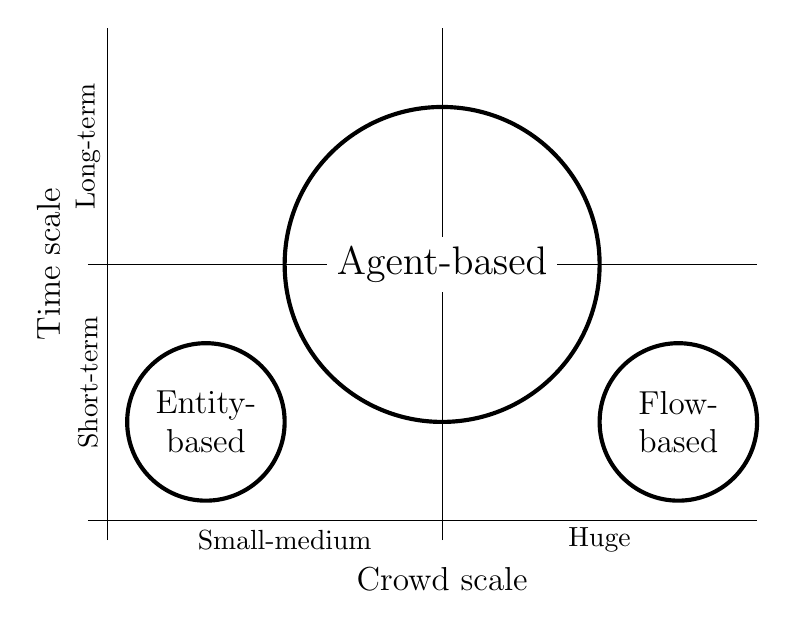
\begin{tikzpicture}[scale=1]
		\draw(4,-0.5) -- (4,6);
		\draw(-0.25,-0.5) -- (-0.25,6);
		\draw(-0.5,3) -- (8,3);
		\draw(-0.5,-0.25) -- (8,-0.25);
		\draw[line width=.15em](4,3)circle(2 and 2)node(A){\Large{\fcolorbox{white}{white}{Agent-based}}};
		\draw[line width=.15em](1,1)circle(1 and 1)node(A){\large\parbox{5em}{\centering Entity-based}};
		\draw[line width=.15em](7,1)circle(1 and 1)node(A){\large\parbox{4em}{\centering Flow-based}};
		\node[rotate=90] at (-0.5,1.5) {Short-term};
		\node[rotate=90] at (-0.5,4.5) {Long-term};
		\node at (2,-0.5) {Small-medium};
		\node at (6,-0.5) {Huge};
		\node[rotate=90] at (-1,3) {\large Time scale};
		\node at (4,-1) {\large Crowd scale};
		\end{tikzpicture}
	  \end{center}

  \caption{\small placeholder figure}
  \label{azahar2}
\end{figure}

\bibliographystyle{plain}
\bibliography{refs}

\end{document}
